\section{Durchführung}
\label{sec:Durchführung}
Für die Durchführung des Versuches wird eine Variation des Michelson-Interferometers verwendet. Der Versuchsaufbau ist \autoref{fig:Aufbau} zu entnehmen.
Vor Beginn der Messung muss das Interferometer so eingestellt werden, dass eine optimale Funktion der Photokathode gewährleistet ist.
Bei eingeschaltetem Laser wird mithilfe der beiden manuell justierbaren Stellschrauben des rechten Spiegels die vertikale und horizontale
Position des Spiegels so eingestellt, dass der auslaufende Lichtstrahl die Linse des Photoelements möglichst genau trifft. Dabei müssen die beiden Teilstrahlen
des Lasers sich überlagern und parallel zueinander verlaufen. Die Stellschraube der vertikalen Justierung wird so eingestellt, dass ein Interferenzmuster
mit möglichst breiten Minima/Maxima entsteht. Wird nun die vom Motor angetriebene Stellschraube gedreht, kann die Photokathode die Interferenz-bedingten
Lichtwechsel registrieren und in ein Zählsignal umwandeln.

\begin{figure}
    \centering
    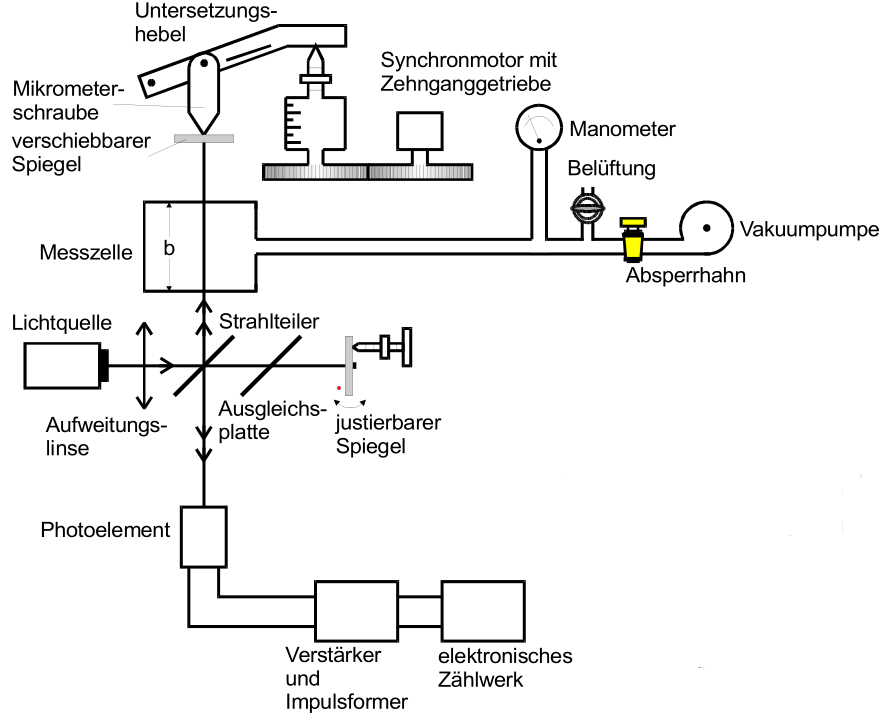
\includegraphics[width = 0.7\textwidth]{content/Aufbau.png}
    \caption{Versuchsaufbau des Experimentes \cite{v401}.}
    \label{fig:Aufbau}
\end{figure}

\subsection{Bestimmung der Wellenlänge des Lasers}
\label{subsec:Laser_Wellenlaenge}
Zur experimentellen Bestimmung der Wellenlänge des verwendeten Lasers wird ein Bereich von $5$ bist $\qty{10}{\milli\metre}$ mit der motorgetriebenen Stellschraube 
abgeschritten. Die Drehzahl des Elektromotors wird auf Stufe $1$ eingestellt. Es werden $10$ Messwerte der Zählraten der Photokathode festgestellt, indem
der oben geannte Messbereich jeweils ein Mal durchschritten wird. Der Zähler der Photokathode wird vor jeder Messung auf $0$ gestellt.
Es ist zu beachten, dass die Stellschraube an einem Hebel mit dem Untersetzungsverhältnis $u = 1:5.046$ wirkt. 
Aus den gewonnenen Messwerten lässt sich ein Mittelwert bilden, aus dem ein experimenteller Wert der Wellenlänge des Lasers folgt.

\subsection{Messung des Brechungsindex von Luft}
\label{subsec:Brechungsindex_Luft}
Um den Brechungsindex der Luft zu bestimmen, wird eine feste Einstellung der Stellschraube gewählt. Diese sollte ebenfalls zwischen $5$ und $\qty{10}{\milli\metre}$
liegen. Durch betätigen der Vakuumpumpe, kann ein Unterdruck in der Messzelle erzeugt werden. Dieser Unterdruck kann am Manometer abgelesen werden.
Es werden 6 Messwerte der Zählraten der Photokathode ermittelt, indem jeweils der Zählstand genullt wird und entweder ein Unterdruck erzeugt wird oder wieder
Luft in die Messzelle gelassen wird. Mithilfe des Wertes des eingestellten Unterdrucks und den Messwerten kann der Brechungsindex von Luft bei den vorherrschenden 
Umgebungsbedingungen ermittelt werden. 
